\section{Data Science}

\todo{It's critical that this section JUSTIFIES THE TOOLS I'm using. Think of a plumber.}

\todo{I'll have to JUSTIFY my approach}

\todo{I'll have to justify why I am selecting certain tools to answer my Research questions. That is the questions in the Diagram in Related Works}

\todo{In addition, extract questions that go into a table. Justify why you have selected the sections and reference the Literature review. Maybe not relevant to my work.}

Data Science is a subset of Computer Science and Mathematics. This subset introduces a new paradigm which creates algorithms for computers and robots. Data Science also involves the use of machine learning algorithms for prediction.


In the field of Data Science, mathematics is very important. This is because principles within mathematics help in the detection of patterns and algorithm construction. In the application of such algorithms in data science, the comprehension of different conceptions of statistics and probability theory is crucial. Notions include Regression, Maximum Likelihood Estimation, distribution's comprehension (Binomial, Bernoulli, Gaussian (Normal)), and Bayes's Theorem.

The foundation of every current field of science is mathematics. Almost all data science methods have a strong mathematical underpinning, like machine learning.
It comes as no surprise that to work as a top data scientist, you would completely need all the other beads of expertise-programming ability, some volume of business intelligence, and your unique analytical and curious mentality-about the data. But learning the machinery under the hood is still worth it, instead of just being the guy behind the wheel with no understanding of the car. A good awareness of the mathematical machinery behind the trendy algorithms would also give you an advantage over your colleagues.

\section{Machine Learning}

Machine Learning is a novel part of Data Science and it encompasses the ability of machines to learn from examples. These models are categorized as either \textbf{\textit{Supervised}} or \textbf{\textit{Unsupervised}} Machine Learning models. 

Although machine learning methods are more concerned with obtaining input/output variables, relational acceptability is still validated with statistical indicators. In GDP studies, several machine/deep learning techniques have been used. The effects of renewable energy production \cite{perera2014machine}, agri-growth conditioned by political stability is analyzed in  employing a huge set of statistical and ML methods. A replication study on the relationship between GDP and oil prices is reported in\cite{charfeddine2020reviewing}

Commodity prices are also the reasonable predictors of GDP. COVID-19 has severely affected even large perpetually stable economies, a deep learning algorithm examined this impact \cite{jena2021impact}. An ANN method is reported in \cite{milavcic2017application}to establish validity of the most used effectors of GDP: services, manufacturing, industrial growth and agri-growth. Deep learning methods are also reported to predict recessions \cite{vrontos2020modeling} and the factors which can affect economic growth negatively.


\subsection{Supervised Learning}
Supervised learning is essentially a formalization of the notion of learning from formerly supervised fields of learning. The learner (usually, a computer programme) is presented with two data sets, a training set and a test set during supervised learning. The idea is to set the learner's training set test to learn 'from a set of classified examples in the training set such that unlabeled examples can be defined with the greatest expected precision in the test set. That is, the learner's goal is to create a law, a programme, or a process that classifies new examples by evaluating examples that already have a class \cite{learned2014introduction}

Supervised learning is further categorized as  either \textbf{\textit{Regression}} or \textbf{\textit{Classification.}} The main difference between Regression and Classification is that the output variable in Regression is numerical while that for Classification is categorical. In other words, Regression predicts a quantity while  Classification predicts a label.


\subsubsection{Machine Learning model - Regression}
In this 1998 article, \cite{zeger1988regression} Scot Zeger posits the analysis of a regression model with a time series. Linear Regression is a basic offshoot of Regression. The predicted output of a Linear Regression model is continuous with a constant slope. The 2 main types of Linear Regression are simple and multivariate regression. 

Simple linear regression can be explained with the slope-intercept form, where \textit{m} and \textit{b} are the variables the algorithm learns to produce the most accurate predictions. \textit{x} in this case represents the input data while \textit{y} the prediction.

\begin{equation}
	y = m x + b
\end{equation}

Multivariate regression is a method with more than one output variable that calculates a single regression model. If a multivariate regression model has more than one predictor variable, the system is a multivariate multiple regression.

A natural extension of multiple linear regression is multivariate linear regression in that both methods aim to explain hypothetical linear correlations between some variables of outputs and inputs. Multiple regression is focused on the analysis of the degree to which a set of "i" input variables X= (X1,Xi) influences the behaviour of a single output variable Y. The multivariate regression has "o" output variables Y= (Y1,Yo), each of which can be affected by precisely the same range of X= (X1,Xi) inputs.\cite{izenman2013multivariate}


\subsubsection{Machine Learning model - Classification}

In this 2006 paper by Kevin P. Murphy \cite{murphy2006naive} he defines a \textbf{classifier} as a function \textit{f} that maps input feature vectors to output classes. This classifier is derived from the \textbf{Bayes' Theorem}

A classification is a tool used to assign groups to a data set in order to assist in detailed forecasts and analysis. You are introduced to an existing data-set with classification algorithms and are aware of the groups of individual instances; with this information, a predictive model can then be created to solve the following problem: For any future instance in the data-set to which a particular instance belongs. Max Entropy, K-Nearest Neighbor, and Naive Bayes are among the types of classification algorithms.



\begin{equation}
	\label{eq:bayes}
	P(\theta | \textbf{D}) = P(\theta ) \frac{P(\textbf{D} |\theta)}{P(\textbf{D})},
\end{equation}



\subsection{Unsupervised Learning}
Unsupervised learning is a category of ML methods that work in the dataset of unlabeled data in order to explore frameworks or trends. New paradigms for unsupervised learning (as such-called self-supervised learning) have also been introduced to manipulate multiple labels that are readily accessible to learn general purpose characteristics in addition to or within visual data.\cite{dayan1999unsupervised}
Unsupervised learning explores how models should learn in a way that illustrates the mathematical form of the overall input sequence set to describe individual input sequence. In comparison to supervised learning or reinforcement learning, each feedback is not correlated with specific goal outcomes or environmental assessments; instead, the unsupervised learning incorporates previous prejudices as to what elements of the input system can be reflected in the output.\cite{dayan1999unsupervised}



\section{Machine Learning Workflow}
One of the fundamental goals of Data Engineering is to develop data pipelines. A Data pipeline means taking data from point A (in an operational system) and then moving it to point B (into something that can be analyzed by data scientists).
The data set used for this thesis paper was gotten from the Food and Agriculture Organization of the United Nations. This organization is tasked with creating a zero-hunger World. Starting from 1945, this organization has amassed a wealth of data-set archives from its member countries all over the world. My focus is on Hungary thus, making my contribution to creating a zero-hunger Hungary.

According to the official website,\cite{division_2000}
\begin{displayquote}
	"FAOSTAT provides free access to food and agriculture data for over 245 countries and territories and covers all FAO regional groupings from 1961 to the most recent year available."
\end{displayquote} 

To achieve my goals I focused on the \textbf{Value Of Agricultural Production} and in particular the \textbf{Gross Production Value.} This value was gotten by multiplying agricultural gross production by the output prices. In the data-sets used in this thesis paper, the gross production value is expressed in US dollars. 



Different data sets are available separately. For the purpose of this thesis, I narrowed down on wheat. I adopted a consistent time-frame. 1965 to 2002. The approach to this was: Given a set of features that are consistent with a particular agricultural product, the aim is to predict the Gross Production Value.

\section{Neural Networks}
A neural network is a collection of algorithms that, through a mechanism that mimics the way the human brain works, aim to identify fundamental connections in a data set \cite{jain1999recurrent}.  Neural networks, in this context, apply to neuron frameworks, either biological or artificial in nature. Machine learning notions have become universally accepted tools in social, pure or applied sciences. Since this work uses neural networks, a note on neural networks will be presented.

\subsection{Biological Neural Network}
Neural networks may respond to evolving inputs, so the network delivers the best possible outcome without the performance parameters having to be revamped. In the development of trading systems, the notion of neural networks, which has its origins in artificial intelligence, is rapidly gaining prominence\cite{krose1993introduction}.


The biological neuron relations are modeled as weights. An excitation relation is reflected by a positive weight, whereas negative values mean inhibitory connections. Each input is updated and summarized by a weight. A linear combination is related to this practice. Finally, the amplitude of the output is regulated by an activation function. A reasonable performance range, for example, is usually between 0 and 1.

\subsection{Artificial Neural Network}

Artificial Neural Networks are applied in regression studies where continuous responses are the most appropriate \cite{haykin2009neural}. They could be of type: feed-forward neural networks (FNN), recurrent neural networks (RNN), convolutional neural networks (CNN), radial-basis functions networks (RBFN) and modular neural networks (MNN) \cite{nielsen2015neural,goyal2013artificial,grossberg2013recurrent,ripley2007pattern}

Some specific examples of research work in agriculture, where neural networks have been employed are presented here. These examples are in addition to the ones mentioned in previous section. In \cite{ghielmi2006descriptive} NNs have been used for crop yield estimation. While in \cite{goyal2013artificial} ANNs have been employed to understand the effects of food security.  

\section{Deep Neural Network}

A recurrent Neural Network(RNN) is a type of Neural Network in which the previous phase output is fed to the current stage as an input. Both the inputs and outputs are independent of each other in conventional neural networks, but in situations such as where it is important to predict the next word of a sentence, the prior words are needed and so the past words need to be recalled. RNN thus came into being, which, with the aid of a Hidden Layer, fixed this problem. Hidden State, which recalls any details about a sequence, is the key and most significant aspect of RNN.\cite{jain1999recurrent}

By giving all layers the same weights and preferences, RNN transforms the independent activation into dependent activation, thereby reducing the difficulty of increasing parameters and memorizing each previous output by giving each output to the next hidden layer as an input.
Therefore, all three layers should be merged into a single recurring layer such that the weights and biases of all the hidden layers are the same.

The formula for calculating the current state:

\[Ht = f(ht-1, Xt)\]

\textit{where} \textbf{H} is the current state, \textbf{ht-1} is the previous state and \textbf{Xt} is the input state.


\subsection{LSTM}
What is LSTM: It's the \textbf{Long short Term Memory} This networks rely on a gated cell to track information throughout many time-steps. How do LSTM work?

\begin{itemize}
	\item Forget: The lSTM forget their irrelevant history.
	
	
	\item Store: They perform computation to store relevant parts of new information.
	
	
	\item Update: They use the above items 1 and 2 to update their internal state.
	
	
	\item Output: Finally, they generate an output.
\end{itemize}

In summary, LSTMs help with uninterrupted gradient flow.

\subsection{Machine Learning vs Deep Learning}

Machine and Deep learning both offer ways to train models and classify data. That is, learning from and classifying previous occurrences. In a standard Machine learning approach, we'll manually select the features in order to train the machine learning model. Those features are then referenced when analyzing and classifying new data. This is the standard workflow to solving a Machine learning problem.

\begin{figure}[h!]
	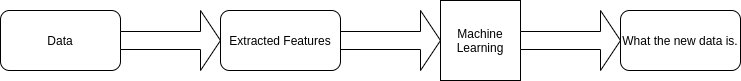
\includegraphics[width=\textwidth,height=\textheight,keepaspectratio]{fig/mlwkflow.png}
	\caption{Machine Learning Workflow}
	\label{fig:ML}
\end{figure}




Deep learning, which is a sub type of Machine learning, on the other hand skips the manual step of extracting features from the data set. Instead, the data is fed directly into the deep learning algorithm which then predicts the required outcome. 

\begin{figure}[H]
	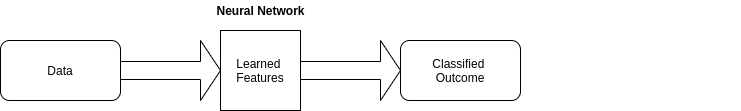
\includegraphics[width=\textwidth]{fig/dpwkflow.png}
	\caption{Deep Learning Workflow}	
	\label{fig:DL}
\end{figure}


In deciding whether to choose Machine or Deep learning, the question to be answered is whether there are lots of labeled data and a high-performance GPU. If these 2 factors are missing, then the right approach would be Machine learning. The reason for this is that Deep learning is generally more complex and highly accurate. One of the downsides to Deep learning is this: because the model is a black box, if something isn't working correctly, it might be hard to debug. 